\documentclass[10pt,a4paper]{article}
\usepackage[T1]{fontenc}
\usepackage[utf8]{inputenc}
\usepackage{lmodern}
\usepackage[margin=20mm,headheight=14pt]{geometry}
\usepackage{graphicx,booktabs,longtable,array,xcolor,amsmath}
\usepackage{fancyvrb,upquote}
\usepackage[hyphens]{url}
\usepackage[colorlinks=true,linkcolor=blue!45!black,urlcolor=blue!45!black,bookmarksnumbered=true,pdfusetitle]{hyperref}
\hypersetup{pdftitle={CoRe: Supplementary Technical Report},pdfauthor={Jingru Yang; Zheng Chen; Ju Fan; Xiaoyong Du}}
\urlstyle{same}
\setlength{\parindent}{0pt}
\setlength{\parskip}{3.5pt plus 1pt}
\setlength{\emergencystretch}{3em}
\renewcommand{\arraystretch}{1.15}
\renewcommand{\thetable}{S\arabic{table}}
\renewcommand{\thefigure}{S\arabic{figure}}
\setcounter{tocdepth}{2}
\newcommand{\ensuretablespace}[1]{\par\ifdim\dimexpr\pagegoal-\pagetotal\relax<#1\relax\newpage\fi}
\setcounter{topnumber}{3}
\setcounter{totalnumber}{4}
\renewcommand{\topfraction}{.95}
\renewcommand{\textfraction}{.02}
\renewcommand{\floatpagefraction}{.80}
\makeatletter\setlength{\@fptop}{0pt}\makeatother
\pagestyle{plain}
\begin{document}
\begin{center}
{\LARGE\bfseries CoRe: Supplementary Technical Report\par}
\vspace{12pt}
{\large Jingru Yang\textsuperscript{1}\quad Zheng Chen\textsuperscript{1}\quad Ju Fan\textsuperscript{2}\quad Xiaoyong Du\textsuperscript{2}\par}
\vspace{5pt}
\textsuperscript{1}Minzu University of China, China\par
\textsuperscript{2}Renmin University of China, China
\end{center}
\vspace{6pt}
\begin{abstract}
This report provides the technical specification and extended evidence for
\emph{Cleaning or Recalling? Disentangling Memorization and World Knowledge in LLM-based Data Cleaning}.
We describe controlled-table construction and acceptance, archived execution and scoring,
Rayyan retrieval and repair-credit criteria, adaptation to other benchmarks, offline
verification routes, extended displays, and sensitivity checks on the existing evidence.
Original inputs, outputs and historical estimates are retained alongside the uniformly re-scored continuation results and exact sign-test corrections. Construction-seed ranges,
fixed-construction bootstrap intervals, and conditional field-audit uncertainty are distinguished throughout.
\end{abstract}
The seven numbered sections correspond to the manuscript's Report \S1--\S7 links.
Tables and figures in this report carry an S prefix; unprefixed numbers refer to the main paper.
Repository links use the canonical source tree at
\href{https://github.com/hinsonver/CoRe-Benchmark/}{hinsonver/CoRe-Benchmark}.
\tableofcontents
\clearpage
\section{Controlled-table construction and acceptance}
\hypertarget{companion-1}{}\label{report-1}

We describe how the four conditions are constructed and checked. The construction preserves paired evidence in the two surrogate conditions while documenting the differences introduced by fresh records.

\subsection{Construction contract}

O is the original benchmark. W and S retain its rows, error cells, chunks and non-identity values, and transfer errors to one-to-one renamed identity values. W uses English words and S uses syllables. F uses other real records with the same schema and error recipes or formatting rules. Its error counts can differ when recipes cannot transfer or a formatting rule applies to more values. These properties support the comparisons in main-paper Section 3.1, not a claim that all four tables have identical repair difficulty.

The construction produces 21 new tables: three conditions (F/W/S) at three seeds for each of Hospital and Movies, plus three Beers conditions at one seed, or 9 + 9 + 3. Together with three original-condition tables, these give 24 cleaning inputs. Conflict inputs and the Rayyan audit are counted separately. The surrogates contain about 41,000 fictitious values. Main sources are \href{https://github.com/hinsonver/CoRe-Benchmark/blob/main/code/src/validate_tables.py}{\nolinkurl{code/src/validate_tables.py}}, the frozen \href{https://github.com/hinsonver/CoRe-Benchmark/blob/main/data/final/}{\nolinkurl{data/final/}} materials, and the paper's \href{https://github.com/hinsonver/CoRe-Benchmark/blob/main/paper/latex/tables/construction.tex}{\nolinkurl{paper/latex/tables/construction.tex}}, \href{https://github.com/hinsonver/CoRe-Benchmark/blob/main/paper/latex/tables/movieserrors.tex}{\nolinkurl{paper/latex/tables/movieserrors.tex}} and \href{https://github.com/hinsonver/CoRe-Benchmark/blob/main/paper/latex/tables/checks.tex}{\nolinkurl{paper/latex/tables/checks.tex}}.

\subsection{Hospital}

The original has 1,000 quality-measure rows for 45 hospitals and 509 erroneous cells. Of these, 508 replace a character by {\ttfamily\small x}; in 96\% of them every occurrence of that character is replaced. Column error rates range from 2.3\% to 3.9\%.

F uses the July 2026 CMS registry. Quality measures are joined with hospital information and converted to the benchmark's 20 columns and formats: lower case, digits-only phone numbers and provider numbers without leading zeros. Whole hospitals are added in provider order, starting with those covered by the benchmark, until 1,000 rows are filled. The table has 34 hospitals, of which 33 occur in O. All quality measures have changed, so these are new rows about largely the same entities. Each column receives the original number of errors, with character substitutions drawn by the original position-weighted rule at newly drawn error locations.

The 296 distinct identity values each map to one fictitious value. S uses 24 syllables and W uses 63 English words, with generic suffixes such as {\ttfamily\small regional hospital} and {\ttfamily\small street}. Provider numbers, ZIP codes and phone numbers become random digits. At each original erroneous position, the transferred corruption replaces a character chosen by position with {\ttfamily\small x}. The small syllable inventory is also the inventory used by the decoding analysis in main-paper Section 8.3; it was not supplied to the cleaner.

\subsection{Movies}

The 1,000-row original subset comprises all 190 rows replaced wholesale by Rotten Tomatoes records and 810 other rows sampled without replacement using Python seed 0. The selected rows retain benchmark order and are restricted to ten columns that IMDb public datasets can fill. Two table-wide formatting rules apply in addition. The 1,965 error cells include 379 identity errors. The complete column breakdown remains in {\ttfamily\small tables/\allowbreak{}movieserrors.tex}.

For example, \emph{American Ultra} (2015) has Rotten Tomatoes slug {\ttfamily\small american\_\allowbreak{}ultra} in place of IMDb identifier {\ttfamily\small tt3316948}, year range {\ttfamily\small 2014 2015 2016}, and Rotten Tomatoes score pair {\ttfamily\small 5.4/\allowbreak{}10,6/\allowbreak{}10} in place of IMDb rating 6.3. Credits can add, omit or respell names. These are source differences, not uniformly typographical errors.

\subsubsection{Fresh film selection and formatting}

For each original film, the constructor selects an absent film from the September 2026 IMDb snapshot. Candidates are feature films with runtime, genres and at least 1,000 votes, released in the same year or, if necessary, within two years. Selection minimizes log-vote-count distance. Clean rows use the first two directors and writers, the first three distinct actors, and durations such as {\ttfamily\small 99 min}.

Fresh row i corresponds to original row i for applying the 190 source-style error recipes. Slugs, year ranges, durations and ratings are instantiated from the original patterns, and the formatting rules are applied to the new values.

\begin{itemize}
\item People recipes record names kept, dropped, respelled or added. Added names come from the fresh film's other columns or other IMDb credits, mirroring the additional names in the other source.
\item Title recipes use the shortest sequence of one or two edits from eleven kinds: capitalization, {\ttfamily\small \&}/{\ttfamily\small and}, accents, punctuation, or added/dropped subtitles, tokens and articles. The error-profile table separately records 12 title edit recipes.
\item Genre recipes preserve the list slots and map the fresh film's genres to Rotten Tomatoes vocabulary, for example {\ttfamily\small Action \& Adventure,Comedy} for {\ttfamily\small Action,Comedy}.
\item A recipe that cannot apply to its assigned fresh cell moves to another source-style row able to take it.
\end{itemize}

Four director and four writer recipes remain inapplicable after relocation. F therefore has 371 identity errors, compared with 379 in O/W/S. At seed 0, F has 2,195 errors overall. Every fresh film has at least 1,000 votes, so the separator rule affects 1,000 rating-count cells rather than 768. These counts describe different fresh records under the same mechanisms, not paired error cells.

\subsubsection{Surrogate names and source-style errors}

The surrogates rename 6,018 values one to one, including 4,018 people. W person names combine English words into first and compound surnames; S person names use two syllable words. Titles are generated independently of the real title, rather than retaining its function words, numbers and punctuation. Generic shapes include {\ttfamily\small The X}, {\ttfamily\small X of the Y}, {\ttfamily\small X: Y Z} and {\ttfamily\small X 2}, sampled at the measured rates: 18.5\% initial {\ttfamily\small The}, 6.1\% colon and 2.9\% final number. W excludes all words appearing in a real title in the table.

Each transferred title error requires a compatible generated shape, such as an {\ttfamily\small and} token or a subtitle. Identifiers become unique fictitious IMDb numbers; the slug is rebuilt from the dirty fictitious title in the form of the original slug. This preserves the corruption mechanism without providing a mapping from a fictitious slug to a random reference identifier.

\subsubsection{Recovery evidence}

The 105 hour/minute duration errors convert to the reference in 50 cases but not in 55; another 80 duration errors are empty and two are other source differences. A format conversion therefore does not always recover the preferred source value. For years, the middle candidate matches 167 of the 190 references. Main-paper Section 7 discusses this candidate-rule example.

\subsection{Beers}

The 1,000-row subset includes all 127 rows with city errors and 873 others sampled without replacement using Python seed 0. Selected rows retain benchmark order. This subset contains 421 breweries, rather than 1,000 independent entities. Its 565 errors comprise 311 percentage suffixes and 254 location cells: a state glued to a city and an empty state cell in each of 127 rows. Correcting the suffix or splitting the location retains the necessary information in the input.

F uses a September 2026 Wikidata query for US beers with alcohol content, style and brewery location. Original beers are excluded, no brewery contributes more than 25 beers, and 1,000 beers from 94 breweries are selected. Corruptions retain the original counts and rendering, including the floating-point representation of percentage values. The original has 421 breweries; F is descriptive in the knowledge analysis because brewery concentration and alcohol-content distributions differ.

Surrogates keep generic words such as {\ttfamily\small Brewing}, {\ttfamily\small Company}, {\ttfamily\small IPA}, {\ttfamily\small Stout} and {\ttfamily\small San}, and years. Other words become W-pool or S-syllable words. Numbers retain their lengths; apostrophes remain only for possessives and {\ttfamily\small O'}. Repeated real values map consistently, including a brewery named for a city. A one-word city remains one word, so a correct generated city does not resemble the city/state-gluing error being tested.

\subsection{Acceptance and construction seeds}

The six check categories contain 67 structural, 137 error-kind/count, 15 error-strength, 263 naming/leakage, 6 fresh-entity and 18 reproducibility checks, totalling 506. Structural checks distinguish paired surrogates from fresh records. Movies column counts generally have an 85\%--115\% tolerance, with error-kind constraints; rating-count errors are checked against the formatting rule. Naming checks include bijection, no original value or title-word reuse, pool membership and title-shape similarity against random pairing.

Eighteen tables are rebuilt under two hash seeds and must match stored files byte for byte. The three main fresh tables use saved source snapshots. The experimental tables pass 505 checks. Hospital W at seed 0 has one/two/at-least-three-character replacement shares of 62.1\%/31.5\%/6.4\%, versus 53.9\%/29.2\%/16.9\% in O. Its largest difference is 10.5 percentage points, 2.5 points beyond the eight-point tolerance. Seeds 1 and 2 pass this check. The error positions remain fixed in all three seeds. The \hyperlink{companion-7}{archived sensitivity checks (Section~\ref{report-7})} give the distributions and condition contrasts separately for the passing seeds. Character-replacement counts describe the corruption profile, rather than a measured model-difficulty scale.

Across construction seeds, surrogates redraw names and applicable transferred-error variants. Fresh tables retain the same clean records and redraw errors and their variants. Thus seed ranges concern naming/error draws, while chunk-bootstrap intervals concern the rows of a fixed construction.
\subsection{Protocol and construction illustrations}
Figures~\ref{report-fig-fig0_overview} and~\ref{report-fig-fig_example_transfer} summarize the protocol and its paired construction example.
\begin{figure}[!htbp]\centering
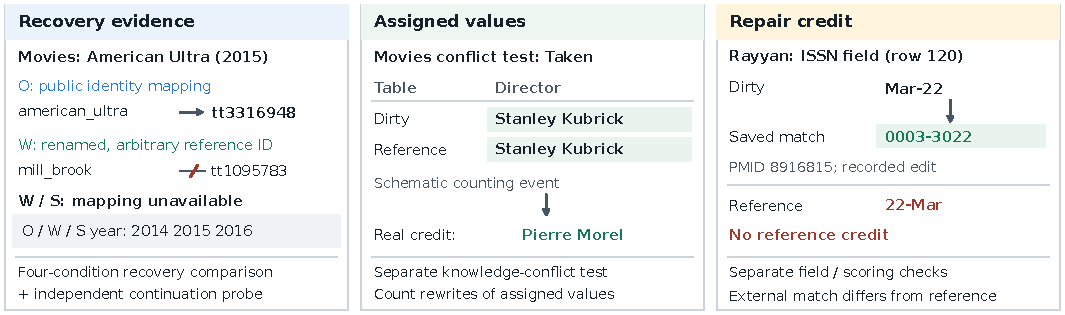
\includegraphics[width=\textwidth,height=.66\textheight,keepaspectratio]{../latex/figures/fig0_overview.pdf}
\caption{Three complementary questions for interpreting repair scores: recovery evidence, preservation of assigned values, and reference credit. The panels illustrate separate tests, not a shared sample.}
\label{report-fig-fig0_overview}
\end{figure}
\begin{figure}[!htbp]\centering
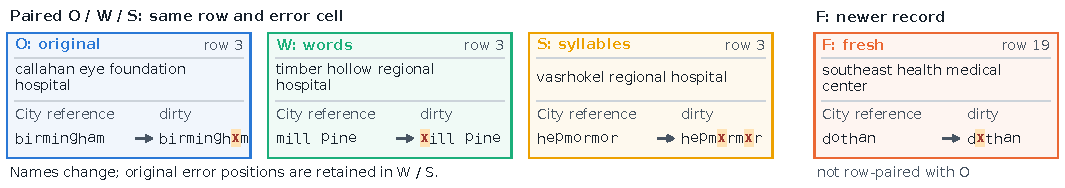
\includegraphics[width=\textwidth,height=.66\textheight,keepaspectratio]{../latex/figures/fig_example_transfer.pdf}
\caption{Hospital construction example. O/W/S share the row and city error position. F uses a newer registry row and a newly drawn error location. Section 6 gives the complete identity fields.}
\label{report-fig-fig_example_transfer}
\end{figure}
\clearpage
\section{Run and scoring specification}
\hypertarget{companion-2}{}\label{report-2}

We specify the archived inputs, model settings, scoring rules and comparison units. The construction contract is in \hyperlink{companion-1}{Construction and acceptance (Section~\ref{report-1})}.

\subsection{Main input and output}

The main direct-editing input contains 20 rows from different entities. Each original and its surrogates share 50 chunks per 1,000-row table. The zero-shot prompt asks for erroneous cells and correct values and asks the model to leave correct cells unchanged; replies are JSON. The aligned setting adds 20 labeled dirty/clean tuples and error positions. Whole-table methods additionally see repeated records of an entity.

\subsection{Models, budgets and incomplete replies}

\ensuretablespace{138pt}
\begingroup\setlength{\tabcolsep}{3pt}\renewcommand{\arraystretch}{1.18}
\small
\begin{longtable}{@{}>{\raggedright\arraybackslash}p{\dimexpr 0.5000\textwidth-3.10pt\relax}>{\raggedright\arraybackslash}p{\dimexpr 0.5000\textwidth-3.10pt\relax}@{}}
\caption{Archived model request and decoding settings.}\label{report-table-2-1}\\
\toprule
Run family & Archived setting \\
\midrule
\endfirsthead
\multicolumn{2}{l}{\small Table \thetable\ (continued)}\\
\toprule
Run family & Archived setting \\
\midrule
\endhead
\midrule\multicolumn{2}{r}{\footnotesize Continued on next page}\\\endfoot
\bottomrule\endlastfoot
DeepSeek-V4-Pro and Qwen3.8-Max & Thinking disabled; requested temperature 0 \\
GLM-5.3 & Reasoning effort low; thinking cannot be disabled; requested temperature 0 \\
GPT-6.1-Sol & Reasoning effort low; client leaves sampling parameters at API defaults \\
Qwen2.5-7B/14B/32B-AWQ Instruct and Llama-3.1-8B-Instruct & Local vLLM and greedy decoding \\
Auxiliary OLMo-2-7B instruction/base variants & Local continuation probe; context limit 4,096 tokens \\
\end{longtable}\endgroup

Replies are capped at 4,096 tokens, except 8,000 for GLM-5.3 and 1,500 for OLMo-2. The client retries replies marked incomplete at twice and four times the budget. Its heuristic checks the final delimiter, rather than an archived API termination reason. Eight of GLM-5.3's 500 Movies replies remain incomplete; all contain only {\ttfamily\small \{"} and parse to no corrections. Their condition distribution and exclusion sensitivity are in \hyperlink{companion-7}{Archived sensitivity checks (Section~\ref{report-7})}. Actual commercial flags are recorded in \href{https://github.com/hinsonver/CoRe-Benchmark/blob/main/code/src/clients.py}{\nolinkurl{code/src/clients.py}}; model-family references do not substitute for those request settings.

The scale statement records about 23,000 prompts: 9,600 zero-shot cleaning prompts, 600 aligned prompts, 3,216 conflict prompts and 9,600 continuation trials. The zero-shot count covers eight models and 24 tables, with 50 chunks per table. These are prompt counts, not a count of independent sampled entities.

\subsection{Method information settings}

Baran receives perfect detection where stated. Its aligned runs use the same chunks, labels and positions as DeepSeek-V4-Pro, averaged over three fixed seeds; whole-table Baran receives repeated records. Baran's Wikipedia-revision value models and Raha's knowledge-base detector are disabled. TabClean uses DeepSeek-V4-Pro, whole tables and 150 sampled development rows, which are excluded from scoring.

The effective TabClean archive contains final outputs and execution logs, not the generated program bodies. All twelve Hospital/Movies/Beers condition outputs have the input shape; the development rows match {\ttfamily\small sample(n=150, random\_\allowbreak{}state=42)} and are excluded from the reported scores. Movies' low identity-column scores accompany successful full-table execution, rather than an aborted run. The available output evidence and effective-version paths are recorded in \hyperlink{companion-6}{Extended displays (Section~\ref{report-6})}.

\subsection{Cell-level scoring}

Let \(E\) be the set of dirty/reference string differences and \(P\) the set of effective edits after no-ops are ignored. The set \(R\subseteq P\cap E\) contains the cells set to the reference value. Repair precision is \(p=|R|/|P|\), recall is \(r=|R|/|E|\), and their harmonic mean is \(F_1=2pr/(p+r)\). Detection replaces \(|R|\) with \(|P\cap E|\) in precision and recall.

The scorer sets precision to zero when \(|P|=0\) and recall to zero when \(|E|=0\). It sets \(F_1=0\) when \(p+r=0\). The same zero-denominator conventions apply to detection. These rules also apply to bootstrap samples containing no errors or no proposed edits; such samples are retained, not dropped. The executable definition is \href{https://github.com/hinsonver/CoRe-Benchmark/blob/main/code/src/probe_clean.py}{\nolinkurl{code/src/probe_clean.py}} (\texttt{metrics}).

No-op and repaired-value comparisons ignore case and normalize whitespace, including spaces around commas. \(E\) uses original strings. Consequently, the five case-only title errors in each Movies condition belong to \(E\) but earn no repair credit under normalized comparison. This convention remains identical across conditions. Identity-column results and other-column results remain separate.

Chunk intervals use 2,000 bootstrap resamples, paired for O/W/S, with 95\% percentile intervals. Bootstrap differences form a Holm family within each result table: the main Hospital/Movies comparison contains 40 differences (eight cleaners times five contrasts). Significance means adjusted p below 0.05. Near-zero results also use repaired-cell counts and paired-chunk sign tests. These sign tests form separate eight-model Holm families for Hospital and Movies, rather than joining the 40 bootstrap differences. The Beers city comparison is another eight-model sign-test family. Its unrounded two-sided binomial p-values enter Holm correction before display rounding. DeepSeek's 10 versus 3 non-tied chunks give adjusted p=0.646; Qwen3.8's 4 versus 15 give 0.154. Both remain non-significant. Seed 0 supplies the main tables. The minimum and maximum over three construction seeds describe naming/error-draw variation, not confidence intervals.

\subsection{Row-continuation probe}

The prompt supplies a header and ten consecutive rows and asks for the next row. It uses 100 trials per dataset for DeepSeek-V4-Pro and 50 for local models, clean or dirty context, with or without dataset names. The six datasets are Hospital, Movies, Beers, Rayyan, Flights and Tax; OLMo-2 omits Movies. The continuation probe covers DeepSeek, the four open-weight cleaners and the two OLMo-2 variants. Qwen3.8-Max, GLM-5.3 and GPT-6.1-Sol are outside this probe's archived coverage. Its absence of positive evidence concerns the tested models and settings.

\textbf{Structural screen.} A hard cell has a target value absent from the corresponding context column and missed by all four structural rules: column mode, most-frequent successor, approximate functional dependencies and previous-value $\pm1$. For clean-context continuation the target is the clean next row; for dirty-context continuation it is the dirty next row. Strictly increasing unit-step counter columns, identified in the clean table, are omitted from cell scoring. This counter exclusion is separate from the $\pm1$ rule applied to other numeric cells.

The rules use the complete source table, including records outside the ten-row prompt. Mode and successor queries subtract one vote for the queried target value; ties retain full-table first-occurrence order. For a dependency $d\to c$, the determinant has at most $N/2$ distinct values, and its modal mapping covers at least 99\% of the $N$ rows. Admission is determined on the full table. A successor query predicts $d$ from its preceding value, then the admitted mapping predicts $c$; the target's mapping vote is subtracted when the predicted determinant equals its actual value. Dependency admission and tie order are not refitted after subtraction. These are offline structural exclusions, not an input-matched cleaner.

\textbf{Parsing and leakage.} Cell-accuracy rates condition on a parsed row. Of 9,600 stored trials, five calls failed, 511 other replies were unparseable, and 9,084 supplied a parsed row. These outcomes remain separate from cell denominators. A clean-value leakage opportunity has an erroneous dirty target whose clean reference is absent from the corresponding dirty-context column. The additional hard-leakage screen uses the full clean table and its clean predecessor. This oracle information may exclude values that the model cannot infer from its dirty prompt. Pooling across settings counts scored cell-trials, not necessarily distinct cells or independent observations.

\textbf{Uniform scoring and results.} Current results apply the complete screen uniformly to the saved replies. Twelve early DeepSeek summaries are compatible with a different counting behavior, without target-vote subtraction or the arithmetic rule; the old source revision was not recovered. Those summaries remain historical records, while the uniform integer counts are stored separately in \href{https://github.com/hinsonver/CoRe-Benchmark/blob/main/results/derived/uniform_continuation.json}{\nolinkurl{results/derived/uniform_continuation.json}}. The current \href{https://github.com/hinsonver/CoRe-Benchmark/blob/main/code/src/uniform_continuation.py}{\nolinkurl{code/src/uniform_continuation.py}} selects maxima and pools leakage from those integers. On Hospital, DeepSeek scores 221/468 (47\%) on context-absent cells and 3/144 (2.1\%) on hard cells. Across tested settings, the largest hard-cell accuracy is 32/375 (0.085 after rounding). OLMo-2 base reaches a displayed maximum of 0.011. Hard clean-value leakage is 3/601 cell-trials for DeepSeek and 1/2,008 for the four open instruction cleaners.

Named and anonymous results are reported separately. Naming can change an individual rate by more than 0.02: Llama's Hospital clean rates are 3/72 and 1/72, a difference of 0.0278. Selecting erroneous target rows can also raise individual screened rates, as with Qwen-7B on Movies dirty (0.0070 to 0.0185). This latter setting changes the sampling pool rather than comparing identical target rows. The public-corpus infini-gram check finds Hospital fragments in a GitHub issue and tool documentation, and none of the other tables.

\textbf{Row-held-out sensitivity.} Removing the target row and both incident transitions, then refitting dependency admission and tie order, gives DeepSeek hard leakage of 3/607. Qwen-7B and Qwen-32B's error-row maxima become 0.028 rather than 0.029. The global maximum 32/375 and Hospital example 3/144 do not change. This separate calculation distinguishes full row-held-out fitting from the target-vote screen used for the reported results. Under the reported screen, the probe supplies no positive evidence attributable to benchmark-row memory beyond the excluded regularities; it does not estimate memory prevalence or rule out contamination.

\subsection{Knowledge-conflict construction and matching}

Targets have assigned attributes in both dirty and reference tables. Exact names, one-vowel-changed names and syllable controls share all other values, error positions and chunk rows. Hospital assignments are consistent across city/state/ZIP/county; Beers across city/state. Movies replaces old surrogate-director occurrences in Creator and Actors with the assigned director in all three versions, avoiding an old-director candidate in another column.

The fixed pool contains 57 films, 24 hospitals and 48 breweries that DeepSeek knows. Main chunks have three targets and 17 other-entity filler rows, with each target appearing once. A supplementary Hospital/Beers setting has three rows per entity, nine target rows and eleven fillers. Known subsets use model-specific factual queries: directors match a credited full name or a surname of at least four letters after accent/punctuation removal; locations require matching city and state code. Known subsets contain 52--57 films, 22--24 hospitals and 7--48 breweries.

The standard prompt asks for cleaning without changing correct cells. The table-evidence prompt adds: ``Base every correction on evidence within this table only. Do not change a value just because it disagrees with what you know about real-world entities.'' Both prompts receive the same chunks and known subsets.

Director rewrites count outputs containing a full credited director name, including films with multiple directors. City rewrites require the normalized real city. The one-letter-name version instead measures restoration of the real name. Matching ignores case and normalizes whitespace; when a cell is listed repeatedly, its last value is scored. Directed matches and any edit to the watched cell are distinct indicators.

The rate first averages row indicators within an entity, then averages over its known entities. With s=1 it is matching films divided by known films; with s=3 it averages the three indicators per entity. Empty or unusable replies remain in the denominator. Controls are scored against the paired real fact with the same target subset. Intervals resample entity means 2,000 times and condition on their fixed table contexts and archived replies.

Executable provenance is in \href{https://github.com/hinsonver/CoRe-Benchmark/blob/main/code/src/near_entities.py}{\nolinkurl{code/src/near_entities.py}}, the archived near-entity runs and the public core's anonymous movie indicators. The exact historical GPT screening dependencies and no-fallback behavior are specified in \href{https://github.com/hinsonver/CoRe-Benchmark/blob/main/docs/gpt-screening.md}{\nolinkurl{docs/gpt-screening.md}} and checked by \href{https://github.com/hinsonver/CoRe-Benchmark/blob/main/tools/check_screening.py}{\nolinkurl{tools/check_screening.py}}.
\clearpage
\section{Rayyan retrieval and repair-credit criteria}
\hypertarget{companion-3}{}\label{report-3}

We describe the Rayyan audit input, title-based retrieval, field-specific checks and repair-credit calculation. The audit retains its saved PubMed matches and the original benchmark reference.

\subsection{Audit input and mechanical transformations}

The audit uses 1,000 rows and eleven columns with 948 dirty/reference differences. All 722 date differences map {\ttfamily\small m/\allowbreak{}d/\allowbreak{}yy} to {\ttfamily\small d/\allowbreak{}int(yy)/\allowbreak{}mm}, with a two-digit input month in the final position: {\ttfamily\small 1/\allowbreak{}1/\allowbreak{}13} to {\ttfamily\small 1/\allowbreak{}13/\allowbreak{}01}, and {\ttfamily\small 5/\allowbreak{}7/\allowbreak{}09} to {\ttfamily\small 7/\allowbreak{}9/\allowbreak{}05}. Of 32 pagination differences, 31 turn ranges into month-name strings, such as {\ttfamily\small 70-6} to {\ttfamily\small Jun-70}.

\subsection{Title-based retrieval}

Sampling draws up to 80 cells per error type with seed 0, including all 75 volume/issue, 32 pagination and twelve ISSN cells, for 279 sampled cells. Queries use the reference title, falling back to the dirty title when empty. The first eight ASCII-letter words longer than three characters are joined with AND in the title field; at least two words are required.

Among up to five candidates, the highest title similarity must reach 0.9. Similarity uses {\ttfamily\small SequenceMatcher} after NFC normalization, case folding, and replacing punctuation and underscores with spaces. There are 152 matched cells and 121 distinct PMIDs. These are automatically selected title matches, not manually certified whole-record matches.

\subsection{Field checks and saved counts}

\ensuretablespace{192pt}
\begingroup\setlength{\tabcolsep}{3pt}\renewcommand{\arraystretch}{1.18}
\small
\begin{longtable}{@{}>{\raggedright\arraybackslash}p{\dimexpr 0.1300\textwidth-4.60pt\relax}>{\raggedright\arraybackslash}p{\dimexpr 0.3800\textwidth-4.60pt\relax}>{\raggedright\arraybackslash}p{\dimexpr 0.2500\textwidth-4.60pt\relax}>{\raggedright\arraybackslash}p{\dimexpr 0.2400\textwidth-4.60pt\relax}@{}}
\caption{Rayyan field-check definitions, population/sample/match counts, and outcomes.}\label{report-table-3-1}\\
\toprule
Check & Definition & Population / sampled / matched & Failed reference / passed dirty \\
\midrule
\endfirsthead
\multicolumn{4}{l}{\small Table \thetable\ (continued)}\\
\toprule
Check & Definition & Population / sampled / matched & Failed reference / passed dirty \\
\midrule
\endhead
\midrule\multicolumn{4}{r}{\footnotesize Continued on next page}\\\endfoot
\bottomrule\endlastfoot
Year & Compare the cell's extracted year with PubMed publication year; 00--26 become 2000--2026 and other two-digit years 1927--1999 & 722 / 80 / 44 & 43 / 42 \\
Changed words & A nonempty set of reference-side changed words must all occur in the PubMed field's case-folded word set; accents remain & 107 / 80 / 38 & 38 / unassessed \\
Volume/issue presence & Reference {\ttfamily\small -1} and dirty empty strings denote absence; compare field availability, not numerical equality & 75 / 75 / 46 & 28 / 17 \\
Pagination & Match the PubMed page string & 32 / 32 / 18 & 18 / 17 \\
ISSN & Accept print or electronic ISSN & 12 / 12 / 6 & 6 / 0 \\
\end{longtable}\endgroup

The date field is {\ttfamily\small article\_\allowbreak{}jcreated\_\allowbreak{}at}; its exact dataset semantics are undocumented, so the test is publication-year consistency. Two reference volumes of {\ttfamily\small 1} pass presence but disagree numerically with saved PubMed volumes {\ttfamily\small 31} and {\ttfamily\small 21} (PMIDs 26452069 and 25819808). Their presence outcomes remain unchanged; the independent numerical differences are carried as annotations. Encoding was checked on the reference side only, hence the unassessed dirty marker.

For each of the five error-type strata \(h\), let \(N_h\) be its population, \(m_h\) its title-matched sample and \(b_h\) the number of failed reference checks. We estimate the weighted failure rate as

\[
\hat{\theta}=\sum_{h=1}^{5}\frac{N_h}{948}\frac{b_h}{m_h}.
\]

The estimate is 95.2\%, with interval 91.2\%--97.8\%. Its weights use the audit input's 948-cell composition. The 722-cell date stratum carries most weight. The 5,000 bootstrap draws resample saved binary outcomes within matched strata with seed 0 and fixed weights. The interval conditions on the selected matches and field criteria, without matching uncertainty or dependence between cells sharing a PMID.

Saved records include query titles, PMIDs, compared field values and outcomes, the publication year for dates, and a text prefix for encoding. Complete candidate responses, returned titles and similarity scores are not retained. A provenance search recovered matching early JSON, logs and programs, but no additional complete candidate-response chain. \href{https://github.com/hinsonver/CoRe-Benchmark/blob/main/code/src/rayyan_audit.py}{\nolinkurl{code/src/rayyan_audit.py}} describes the historical query/check logic; the public replay uses saved matches and outcomes rather than issuing fresh searches.

\subsection{Repair credit and input versions}

On the audit input, DeepSeek zero-shot output scores F1 0.002. At zero-based row 120, dirty ISSN {\ttfamily\small Mar-22} becomes output {\ttfamily\small 0003-3022}, matching saved PMID 8916815, while the reference is {\ttfamily\small 22-Mar}. This output gets no benchmark repair credit.

TabClean's distributed input has 960 differences. It removes commas, represents empty values as {\ttfamily\small empty}, and has twelve additional dirty-side error positions. Both inputs have 1,000 rows and eleven columns and share the date-conversion pattern. Scoring uses the actual TabClean pair, not the audit pair, and removes the 150 development rows sampled with {\ttfamily\small random\_\allowbreak{}state=42}.

The remaining 850 rows have 808 errors. There are 498 effective edits and 461 credited repairs, so {\ttfamily\small F1=2*461/\allowbreak{}(498+808)=0.71} after rounding. Of the 461 credited repairs, 434 (94\%) reproduce the reference date transformation. This is a count of credited output transformations, not a claim about the method's intent or a new externally rescored ranking.

The public entry is \href{https://github.com/hinsonver/CoRe-Benchmark/blob/main/tools/check_rayyan.py}{\nolinkurl{tools/check_rayyan.py}}; it binds audit and TabClean inputs, development indices and output to the recorded versions. See \href{https://github.com/hinsonver/CoRe-Benchmark/blob/main/docs/rayyan-replay.md}{\nolinkurl{docs/rayyan-replay.md}} and \hyperlink{companion-5}{Public verification (Section~\ref{report-5})}.

\subsection{Other reference examples}

Hospital assigns Helen Keller Memorial Hospital in Sheffield, Alabama to Jefferson County in 25 rows, although Sheffield is in Colbert County. Qwen3.8-Max, GLM-5.3 and GPT-6.1-Sol correct 10, 11 and 21 such cells, each scored as a false edit. Movies repeats the same writer in 68 reference cells, for example {\ttfamily\small Andrew Smith,Andrew Smith}. These examples retain the original benchmark scoring and do not replace the frozen results.
\clearpage
\section{Applying CoRe to another benchmark}
\hypertarget{companion-4}{}\label{report-4}

We describe how to adapt CoRe to another benchmark, starting from the evidence available for recovering each error. These recommendations extend the evaluation design, not the empirical coverage of the present study.

\subsection{Identity columns and recovery evidence}

Identify columns whose values name or locate an entity. Before constructing variants, profile each column's error kinds, strengths, positions and table-wide rules. For each kind, record what the shown input retains: a reversible format, candidates or regularities, or a value requiring additional evidence. The same column can contain more than one case, and examples or repeated records can change recoverability.

\subsection{Fresh records}

Select a source of the same kind and map it to the benchmark schema and formatting. Document what has changed: records, entities, value distributions and error composition. Reapply error recipes to the new records and record cases that cannot transfer. Fresh records complement paired substitutions; they are not a substitute for them or automatically free of familiar entities.

\subsection{Two naming styles}

Construct one-to-one English-word and syllable replacements. Retain generic terms and column conventions while avoiding real-value reuse, title-shape leakage and names that resemble the errors being tested. Keep non-identity values and error positions fixed in surrogates. Transfer the error mechanism rather than generating an unrelated corruption.

\subsection{Acceptance and seeds}

Encode structural, error-profile, naming/leakage and source-selection requirements as checks. Rebuild code-generated tables to test determinism and retain source snapshots for externally acquired fresh tables. Record exceptions explicitly. Use construction seeds to expose naming/error sensitivity, separating it from bootstrap variation over a fixed table. State which clean records are held fixed across seeds.

\subsection{Fair comparisons and value preservation}

Hold prompts, available labels, error positions and access to repeated records fixed within a comparison. Define cell-level scoring and the reference source. Add a separate continuation test with structural baselines when interpreting possible memorization. For conflicting facts, specify assigned values to preserve, pair name variants, identify each model's known subset, and measure directed factual rewrites separately from other edits.

\subsection{Cost and scope}

Most adaptation effort lies in error profiling and transferable recipes. Single-character typos require less source-specific handling than cross-source titles, credits, ratings and genres. A successful transfer needs a stated source convention and available recovery evidence, not just renamed entities. Matching and imputation are potential future settings, rather than tasks already validated by the present study.

Implementation details for the current study are in \hyperlink{companion-1}{Construction (Section~\ref{report-1})}, \hyperlink{companion-2}{Runs and scoring (Section~\ref{report-2})} and \hyperlink{companion-3}{Rayyan checks (Section~\ref{report-3})}.
\clearpage
\section{Evidence and offline verification}
\hypertarget{companion-5}{}\label{report-5}

This guide maps the manuscript's analyses to the included evidence and executable replay routes. It distinguishes the current manuscript presentation from the earlier fixed statistical ZIP.

The current repository presentation produces 19 table sources (17 full sources and two compact views) and eleven CSV files. It includes the focused recovery comparison and Hospital construction example. The earlier fixed statistical package, {\ttfamily\small CoRe-public-core-statistical.zip}, retains 16 table sources and nine CSV files. Its SHA-256 is {\ttfamily\small 9a4e03a3\allowbreak{}af74696f\allowbreak{}2e100fc1\allowbreak{}a12b0831\allowbreak{}f718cf67\allowbreak{}6a5a5b5d\allowbreak{}e7d4e054\allowbreak{}c86542d0}, and its manifest SHA-256 is {\ttfamily\small 3162d8b7\allowbreak{}e9433728\allowbreak{}40c1960a\allowbreak{}5f7fc2c2\allowbreak{}57c7f376\allowbreak{}8e6baa9c\allowbreak{}75e47cdb\allowbreak{}5fa32f38}. These historical bindings are not replaced by the current presentation. The current first figure contrasts saved Movies identifier-mapping counts with retained year candidates; the original three-dataset overview and intervals remain in the extended displays.

\subsection{Public offline entry}

Use the dependencies in \href{https://github.com/hinsonver/CoRe-Benchmark/blob/main/environment/requirements.txt}{\nolinkurl{environment/requirements.txt}}. From the repository root, with a new output path:

\begin{quote}
\begin{Verbatim}[fontsize=\footnotesize,fontfamily=cmtt,formatcom={\fontencoding{OT1}\selectfont\def\textasciigrave{\char18}\def\textquotesingle{\char13}}]
python3 tools/core.py verify
python3 tools/core.py reproduce --output /new/public-results
python3 tools/check_rayyan.py
python3 tools/review_diagnostics.py
\end{Verbatim}
\end{quote}

The \href{https://github.com/hinsonver/CoRe-Benchmark/blob/main/scripts/verify.sh}{\nolinkurl{scripts/verify.sh}} and \href{https://github.com/hinsonver/CoRe-Benchmark/blob/main/scripts/reproduce.sh}{\nolinkurl{scripts/reproduce.sh}} wrappers use the selected {\ttfamily\small PYTHON} interpreter. Public replay requires no GPU, model key or network. The current presentation regenerates 19 table sources and eleven CSV files, using uniform continuation counts and exact sign-test probabilities before Holm correction. Adding {\ttfamily\small --presentation frozen} selects the original archived scores and formatting. The fixed ZIP's 16-table/nine-CSV inventory describes that historical archive, not the current presentation. Explanatory verification and diagram views are not additional experimental observations.

\subsection{Manuscript to evidence map}

All package paths below are relative to its extracted root. Generated paths are relative to the requested output directory.

\ensuretablespace{245pt}
\begingroup\setlength{\tabcolsep}{3pt}\renewcommand{\arraystretch}{1.18}
\small
\begin{longtable}{@{}>{\raggedright\arraybackslash}p{\dimexpr 0.1600\textwidth-4.60pt\relax}>{\raggedright\arraybackslash}p{\dimexpr 0.3100\textwidth-4.60pt\relax}>{\raggedright\arraybackslash}p{\dimexpr 0.2100\textwidth-4.60pt\relax}>{\raggedright\arraybackslash}p{\dimexpr 0.3200\textwidth-4.60pt\relax}@{}}
\caption{Evidence and executable replay routes by analysis.}\label{report-table-5-1}\\
\toprule
Analysis and manuscript labels & Public evidence & Entry & Replayed products \\
\midrule
\endfirsthead
\multicolumn{4}{l}{\small Table \thetable\ (continued)}\\
\toprule
Analysis and manuscript labels & Public evidence & Entry & Replayed products \\
\midrule
\endhead
\midrule\multicolumn{4}{r}{\footnotesize Continued on next page}\\\endfoot
\bottomrule\endlastfoot
Knowledge effects and continuation & Archived block counts and construction summaries; uniform continuation integer counts; \href{https://github.com/hinsonver/CoRe-Benchmark/blob/main/data/witnesses/movies.json}{\nolinkurl{data/witnesses/movies.json}}; original evidence under \href{https://github.com/hinsonver/CoRe-Benchmark/blob/main/artifacts/raw_outputs/p2/}{\nolinkurl{artifacts/raw_outputs/p2/}}, {\ttfamily\small p1/\allowbreak{}}, {\ttfamily\small aligned/\allowbreak{}}, {\ttfamily\small e4/\allowbreak{}}, {\ttfamily\small e5/\allowbreak{}} & \href{https://github.com/hinsonver/CoRe-Benchmark/blob/main/scripts/reproduce.sh}{\nolinkurl{scripts/reproduce.sh}} or {\ttfamily\small tools/\allowbreak{}core.py reproduce} & Contrasts, block-bootstrap intervals, significance, seed/scale summaries, aligned results and figure CSVs. Current continuation maxima and leakage use separately bound uniform counts. \\
Knowledge conflicts & Anonymous movie entity IDs, per-model known flags and directed/any-edit indicators; Hospital/Beers archived conflict results & {\ttfamily\small tools/\allowbreak{}core.py verify} and public reproduce & Full/known entity-bootstrap checks, {\ttfamily\small tables/\allowbreak{}near.tex}, {\ttfamily\small conflictcounts.tex}, {\ttfamily\small fig4\_\allowbreak{}near\_\allowbreak{}entity.csv}, {\ttfamily\small fig7\_\allowbreak{}near\_\allowbreak{}models.csv}; retains known denominators and control edits. \\
Reference quality and repair credit & Saved title matches and field checks, \href{https://github.com/hinsonver/CoRe-Benchmark/blob/main/data/manifests/RAYYAN_REPLAY.json}{\nolinkurl{data/manifests/RAYYAN_REPLAY.json}}, {\ttfamily\small results/\allowbreak{}derived/\allowbreak{}rayyan\_\allowbreak{}audit.json}, \href{https://github.com/hinsonver/CoRe-Benchmark/blob/main/data/provenance/rayyan/}{\nolinkurl{data/provenance/rayyan/}}, audit and actual TabClean inputs, development indices and archived output & \href{https://github.com/hinsonver/CoRe-Benchmark/blob/main/tools/check_rayyan.py}{\nolinkurl{tools/check_rayyan.py}}; public reproduce also invokes it & Weighted check-failure estimate/interval, {\ttfamily\small derived/\allowbreak{}rayyan\_\allowbreak{}replay.json}, {\ttfamily\small tables/\allowbreak{}rayyan.tex}, Rayyan CSVs and the 808/498/461/434 scoring counts. \\
\end{longtable}\endgroup

Movie witnesses contain numerical projections, not row-level movie values or replies. {\ttfamily\small CORE\_\allowbreak{}WITNESSES.json} binds projections and {\ttfamily\small CORE\_\allowbreak{}SOURCES.json} records historical local-validation dependencies. Rayyan replay uses saved matches and scalar checks, with saved encoding outcomes, rather than a fresh PubMed retrieval. Beers F provenance has the additional entry {\ttfamily\small python3 supplements/\allowbreak{}beers-f-input-provenance/\allowbreak{}verify.py}.

\subsection{Current manuscript display projections}

The current manuscript uses the full {\ttfamily\small tables/\allowbreak{}aligned.tex} matrix and full eight-model scale plot. {\ttfamily\small tables/\allowbreak{}rayyan\_\allowbreak{}checks.tex} combines the original sampling counts with the five matched-cell check fractions. The unused six-row {\ttfamily\small tables/\allowbreak{}whole\_\allowbreak{}table.tex} projection and original Rayyan count table/plot remain in \hyperlink{companion-6}{extended displays (Section~\ref{report-6})}. Figure 6 and all its plotted intervals are unchanged.

The first figure's saved numerators are in \href{https://github.com/hinsonver/CoRe-Benchmark/blob/main/paper/latex/tables/moviescols.tex}{\nolinkurl{paper/latex/tables/moviescols.tex}} and cross-checked against the original year CSV. Its generator is \href{https://github.com/hinsonver/CoRe-Benchmark/blob/main/code/src/evidence_panels.py}{\nolinkurl{code/src/evidence_panels.py}}. The overview and Hospital construction figure explain the protocol using existing examples; they add no experimental observations. Their generator is \href{https://github.com/hinsonver/CoRe-Benchmark/blob/main/code/src/example_diagrams.py}{\nolinkurl{code/src/example_diagrams.py}}, called from \href{https://github.com/hinsonver/CoRe-Benchmark/blob/main/code/src/figures.py}{\nolinkurl{code/src/figures.py}}. PDF, PNG, SVG and source-cell CSV exports are retained. The complete Hospital identity-field table remains in the extended displays.

The checked table-display entry is \href{https://github.com/hinsonver/CoRe-Benchmark/blob/main/code/src/paper_presentation.py}{\nolinkurl{code/src/paper_presentation.py}}. The current repository replay invokes this projection, checks all 17 full source bodies, overlays current captions and adds two compact sources. The projection does not retroactively alter the earlier fixed ZIP.

\subsection{Authorized historical movie validation}

Readers supplying the exact historical inputs, replies and scoring code can use:

\begin{quote}
\begin{Verbatim}[fontsize=\footnotesize,fontfamily=cmtt,formatcom={\fontencoding{OT1}\selectfont\def\textasciigrave{\char18}\def\textquotesingle{\char13}}]
python3 tools/core.py validate-private \
  --private-root /external/historical-root \
  --authorization-record /external/rights-record.json \
  --output /new/historical-validation-results
\end{Verbatim}
\end{quote}

The authorization record contains {\ttfamily\small purpose}, {\ttfamily\small rights\_\allowbreak{}basis}, a {\ttfamily\small scope} with {\ttfamily\small historical\_\allowbreak{}inputs} and {\ttfamily\small historical\_\allowbreak{}outputs}, and {\ttfamily\small redistribution: false}. The entry checks 264 historical dependencies and 25 code files against the manifest before re-scoring saved direct-editing, aligned and conflict replies. Its witnesses must match the public witnesses. The original continuation summaries remain available in frozen replay; the current presentation uses the separately bound uniform counts described in Section 2.5. The raw continuation scoring entry checks the stored replies when the corresponding inputs are available. New daily IMDb downloads or new model replies do not replace the historical materials.

\subsection{Verification boundaries}

The seven sections of the supplementary technical report give construction, execution, Rayyan criteria, adaptation guidance, replay routes, extended displays and diagnostic detail. Offline reproducibility does not imply redistribution of excluded historical movie records or access to model services. {\ttfamily\small verify --release} additionally checks citation metadata and an external approval record bound to the final manifest; these are release checks rather than statistical evidence.
\clearpage
\section{Extended displays and result details}
\hypertarget{companion-6}{}\label{report-6}

This material accompanies the current manuscript. It retains the complete Hospital example, three-dataset condition overview, aligned/whole-table matrix, full acceptance table and original Rayyan display. All values come from the frozen sources.

\subsection{Three-dataset condition overview}

The \href{https://github.com/hinsonver/CoRe-Benchmark/blob/main/paper/latex/figures/fig1_decomposition.pdf}{original overview plot} and \href{https://github.com/hinsonver/CoRe-Benchmark/blob/main/results/figures/fig1_decomposition.csv}{complete plotted CSV} retain DeepSeek-V4-Pro's four-condition repair F1 on Hospital/Movies identity columns and all Beers columns, including the original 95\% chunk-bootstrap intervals. O/W/S are paired; F uses fresh real records. Beers F is descriptive because brewery concentration and alcohol-content distributions differ. No point estimate, interval or CSV row is replaced by the focused first figure.

The main-paper Figure 1 instead contrasts Movies identifier mappings with retained year candidates, using existing repaired/error counts from Table 10. It does not introduce a new significance test or interval estimate. Figure 4 retains the detailed distribution of year choices; the middle-year rule matches 167/190 references and was not supplied to the zero-shot cleaner.

\subsection{Hospital row across four conditions}

Hospital identity fields across conditions, with the corrupted city in bold. O/W/S share a row and error position. F draws a newer registry row with updated quality measures rather than a row-paired replacement of O.

\ensuretablespace{138pt}
\begingroup\setlength{\tabcolsep}{3pt}\renewcommand{\arraystretch}{1.18}
\footnotesize
\begin{longtable}{@{}>{\raggedright\arraybackslash}p{\dimexpr 0.0800\textwidth-5.10pt\relax}>{\raggedright\arraybackslash}p{\dimexpr 0.2350\textwidth-5.10pt\relax}>{\raggedright\arraybackslash}p{\dimexpr 0.2000\textwidth-5.10pt\relax}>{\raggedright\arraybackslash}p{\dimexpr 0.1700\textwidth-5.10pt\relax}>{\raggedright\arraybackslash}p{\dimexpr 0.1500\textwidth-5.10pt\relax}>{\raggedright\arraybackslash}p{\dimexpr 0.1650\textwidth-5.10pt\relax}@{}}
\caption{Hospital identity fields across the four conditions; bold cities are corrupted.}\label{report-table-6-1}\\
\toprule
Version & Name & Address & City & County & Phone \\
\midrule
\endfirsthead
\multicolumn{6}{l}{\small Table \thetable\ (continued)}\\
\toprule
Version & Name & Address & City & County & Phone \\
\midrule
\endhead
\midrule\multicolumn{6}{r}{\footnotesize Continued on next page}\\\endfoot
\bottomrule\endlastfoot
O & callahan eye foundation hospital & 1720 university blvd & \textbf{birminghxm} & jefferson & 2053258100 \\
F & southeast health medical center & 1108 ross clark circle & \textbf{dxthan} & houston & 3347938701 \\
W & timber hollow regional hospital & 5749 glen road & \textbf{xill pine} & sunset prairie & 6175712390 \\
S & vasrhokel regional hospital & 8928 zarquen street & \textbf{hepmxrmxr} & lotorcal & 6061657772 \\
\end{longtable}\endgroup

The \href{https://github.com/hinsonver/CoRe-Benchmark/blob/main/paper/latex/tables/example.tex}{complete original table source} retains all six columns above. Main-paper Figure 3 focuses on hospital names and the clean-to-dirty city transfer, with F separated from paired O/W/S. Its reference/dirty city pairs are {\ttfamily\small birmingham}/{\ttfamily\small birminghxm}, {\ttfamily\small mill pine}/{\ttfamily\small xill pine}, {\ttfamily\small hepmormor}/{\ttfamily\small hepmxrmxr}, and {\ttfamily\small dothan}/{\ttfamily\small dxthan}, respectively. Hospital F contains 34 hospitals, 33 shared with O, with updated quality measures and newly drawn error locations.

\subsection{Acceptance checks}

The 506 checks cover 21 tables. The \href{https://github.com/hinsonver/CoRe-Benchmark/blob/main/paper/latex/tables/checks.tex}{complete table source} preserves the original categories and operations.

\ensuretablespace{181pt}
\begingroup\setlength{\tabcolsep}{3pt}\renewcommand{\arraystretch}{1.18}
\small
\begin{longtable}{@{}>{\raggedright\arraybackslash}p{\dimexpr 0.2200\textwidth-4.10pt\relax}>{\raggedright\arraybackslash}p{\dimexpr 0.1400\textwidth-4.10pt\relax}>{\raggedright\arraybackslash}p{\dimexpr 0.6400\textwidth-4.10pt\relax}@{}}
\caption{Construction acceptance checks by category.}\label{report-table-6-2}\\
\toprule
Category & Checks & What is checked \\
\midrule
\endfirsthead
\multicolumn{3}{l}{\small Table \thetable\ (continued)}\\
\toprule
Category & Checks & What is checked \\
\midrule
\endhead
\midrule\multicolumn{3}{r}{\footnotesize Continued on next page}\\\endfoot
\bottomrule\endlastfoot
Structure & 67 & Shape and columns; error cells where the original has them; identical non-identity cells; different seeds with shared fresh clean tables. \\
Error kinds and counts & 137 & Per-column kinds and counts as in the original; formatting rules; errors only in rows that carry them. \\
Error strength & 15 & Characters replaced per error cell within the tolerance of the original. \\
Naming and leakage & 263 & One fictitious value per real value and back; no real value reused; no word of a real title; title shapes no closer to real ones than chance; names that look like names. \\
Fresh entities & 6 & No benchmark entity where new entities are required; locations checked against sources. \\
Reproducibility & 18 & Every table rebuilt byte for byte under two hash seeds. \\
\end{longtable}\endgroup

The checks follow each family's fresh-source design: Hospital F uses newer rows largely about the same institutions. The tables pass 505/506 checks. Hospital W at seed 0 has a maximum error-strength difference of 10.5 percentage points, exceeding the eight-point tolerance by 2.5 points. Seeds 1 and 2 pass, with all error positions unchanged. \hyperlink{companion-1}{Construction and acceptance (Section~\ref{report-1})} gives the thresholds; \hyperlink{companion-7}{Archived sensitivity checks (Section~\ref{report-7})} give the passing-seed contrasts without replacing the frozen main table.

\subsection{Aligned and whole-table repair}

Identity-column repair F1 is shown below in full and in main-paper Table 13. Aligned methods receive the same chunks, 20 labeled tuples and error positions. Baran is the mean of three runs; whole-table Baran uses perfect detection. TabClean uses DeepSeek-V4-Pro with development rows excluded. The \href{https://github.com/hinsonver/CoRe-Benchmark/blob/main/paper/latex/tables/aligned.tex}{complete table source} retains all twelve method/dataset rows.

\ensuretablespace{192pt}
\begingroup\setlength{\tabcolsep}{3pt}\renewcommand{\arraystretch}{1.18}
\footnotesize
\begin{longtable}{@{}>{\raggedright\arraybackslash}p{\dimexpr 0.1800\textwidth-5.10pt\relax}>{\raggedright\arraybackslash}p{\dimexpr 0.3000\textwidth-5.10pt\relax}>{\raggedright\arraybackslash}p{\dimexpr 0.1300\textwidth-5.10pt\relax}>{\raggedright\arraybackslash}p{\dimexpr 0.1300\textwidth-5.10pt\relax}>{\raggedright\arraybackslash}p{\dimexpr 0.1300\textwidth-5.10pt\relax}>{\raggedright\arraybackslash}p{\dimexpr 0.1300\textwidth-5.10pt\relax}@{}}
\caption{Identity-column repair F1 under aligned and whole-table information.}\label{report-table-6-3}\\
\toprule
Dataset & Method & O & F & W & S \\
\midrule
\endfirsthead
\multicolumn{6}{l}{\small Table \thetable\ (continued)}\\
\toprule
Dataset & Method & O & F & W & S \\
\midrule
\endhead
\midrule\multicolumn{6}{r}{\footnotesize Continued on next page}\\\endfoot
\bottomrule\endlastfoot
Hospital & DeepSeek, aligned & 0.97 & 0.98 & 0.76 & 0.75 \\
Hospital & Baran, aligned & 0.29 & 0.32 & 0.27 & 0.28 \\
Hospital & Baran, whole table & 0.91 & 0.93 & 0.93 & 0.93 \\
Hospital & TabClean & 1.00 & 1.00 & 0.96 & 0.99 \\
Movies & DeepSeek, aligned & 0.64 & 0.67 & 0.09 & 0.07 \\
Movies & Baran, aligned & 0.00 & 0.00 & 0.00 & 0.00 \\
Movies & Baran, whole table & 0.27 & 0.26 & 0.26 & 0.25 \\
Movies & TabClean & 0.00 & 0.00 & 0.03 & 0.00 \\
Beers & DeepSeek, aligned & 1.00 & 1.00 & 1.00 & 1.00 \\
Beers & Baran, aligned & 0.19 & 0.77 & 0.20 & 0.22 \\
Beers & Baran, whole table & 0.94 & 1.00 & 0.94 & 0.96 \\
Beers & TabClean & 1.00 & 1.00 & 1.00 & 1.00 \\
\end{longtable}\endgroup

Main-paper Figure 6 displays Hospital/Movies zero-shot and aligned results with intervals, using all 24 rows of \href{https://github.com/hinsonver/CoRe-Benchmark/blob/main/results/figures/fig3_aligned.csv}{the plotted CSV}. Table 13 supplies exact scores across both information settings, including Beers. All three families use identity-column scoring here. For aligned Baran, each plotted whisker is the first run's 95\% chunk-bootstrap interval translated by the difference between the three-run mean and the first run's point estimate. It is neither a confidence interval for the three-run mean nor an interval over seeds. The implementation is \href{https://github.com/hinsonver/CoRe-Benchmark/blob/main/code/src/figures.py}{\nolinkurl{code/src/figures.py}} (\texttt{fig3}), and the CSV retains the exact plotted endpoints. The earlier six-row projection, \href{https://github.com/hinsonver/CoRe-Benchmark/blob/main/paper/latex/tables/whole_table.tex}{\nolinkurl{whole_table.tex}}, is retained as an unused generated view rather than an additional main-paper table.

Whole-table Baran and TabClean combine high scores with little change under renaming on Hospital and Beers. Movies has a different profile: whole-table Baran remains at 0.25--0.27, while TabClean is at 0.00--0.03. The latter's small variation accompanies almost no identity repairs, rather than successful recovery across names. Aligned Baran also remains at zero on Movies. These cases are kept separate from the high-score comparisons in Finding 5.

\subsection{Rayyan: original plot and counts}

Main-paper Table 17 combines the original population, sampling and title-match counts with reference-failure and dirty-pass fractions. \href{https://github.com/hinsonver/CoRe-Benchmark/blob/main/paper/latex/tables/rayyan.tex}{The original count table}, \href{https://github.com/hinsonver/CoRe-Benchmark/blob/main/paper/latex/figures/fig5_rayyan.pdf}{original plot}, \href{https://github.com/hinsonver/CoRe-Benchmark/blob/main/results/figures/fig5_rayyan.csv}{count CSV} and \href{https://github.com/hinsonver/CoRe-Benchmark/blob/main/results/figures/fig5_rayyan_display.csv}{display CSV} are retained. The changed-words dirty check is unassessed, not zero.

The field definitions and conditional weighted estimate are specified in \hyperlink{companion-3}{Rayyan retrieval and scoring details (Section~\ref{report-3})}. The plot and the revised table use the same five strata and matched cells; they are not separate samples.

\subsection{Full model comparison and presentation generation}

The \href{https://github.com/hinsonver/CoRe-Benchmark/blob/main/paper/latex/figures/fig6_scale.pdf}{full eight-model scale plot} and \href{https://github.com/hinsonver/CoRe-Benchmark/blob/main/results/figures/fig6_scale.csv}{frozen scale CSV} remain available. Any focused main-paper view selects original rows and intervals without re-estimation.

The current presentation checks the non-caption content of its bound table sources, restores the manuscript captions, and adds {\ttfamily\small whole\_\allowbreak{}table.tex} and {\ttfamily\small rayyan\_\allowbreak{}checks.tex}. Its continuation table uses the uniform integer counts in Section 2.5, and its Beers city tests apply Holm to unrounded probabilities. The original archived scores remain available under {\ttfamily\small --presentation frozen}. Current replay produces 19 table sources and eleven CSV files:

\begin{quote}
\begin{Verbatim}[fontsize=\footnotesize,fontfamily=cmtt,formatcom={\fontencoding{OT1}\selectfont\def\textasciigrave{\char18}\def\textquotesingle{\char13}}]
python3 tools/core.py reproduce --output /new/public-results
\end{Verbatim}
\end{quote}

The earlier fixed statistical ZIP retains its 16-table/nine-CSV inventory and original hashes. The current presentation and historical ZIP are distinct versioned deliverables, as described in \hyperlink{companion-5}{Public verification (Section~\ref{report-5})}.

\subsection{TabClean: archived output evidence}

The effective TabClean archive is \href{https://github.com/hinsonver/CoRe-Benchmark/blob/main/artifacts/raw_outputs/e4/}{\nolinkurl{artifacts/raw_outputs/e4/}}. Historical {\ttfamily\small \_\allowbreak{}failed\_\allowbreak{}1001}, {\ttfamily\small \_\allowbreak{}fresh\_\allowbreak{}v2}, {\ttfamily\small \_\allowbreak{}movies\_\allowbreak{}v2\_\allowbreak{}1002} and {\ttfamily\small \_\allowbreak{}beers\_\allowbreak{}v3\_\allowbreak{}1002} directories are not substituted for these final files. The effective archive retains the final condition outputs and execution evidence.

All twelve reported condition outputs have successful full-table execution logs. The 150 development rows match {\ttfamily\small sample(n=150, random\_\allowbreak{}state=42)} and are excluded from the scores. On Movies, the original, fresh, word and syllable conditions repair 0, 0, 5 and 0 identity cells, respectively, out of 319, 313, 319 and 319 errors after exclusion. These counts explain the displayed near-zero F1 values without treating the runs as aborted executions.

For a Beers example outside the development rows, {\ttfamily\small San Francisco CA} in City and an empty State become {\ttfamily\small San Francisco} and {\ttfamily\small CA}, matching the reference. Both pieces of information are present in the dirty input. All 104 non-development city-error rows in Beers O have the correct city and state in the final output. The generated program bodies were not retained in this effective archive, so the example describes observed edits, not a recovered internal rule. The archived outputs and \href{https://github.com/hinsonver/CoRe-Benchmark/blob/main/code/src/e4.py}{\nolinkurl{code/src/e4.py}} specify the effective versions and development exclusions.
\subsection{Exact aligned-Baran plotting endpoints}
Table~\ref{report-table-6-4} gives the unmodified CSV endpoints for the Baran series in main-paper Figure 6. The center is a three-run mean. The whiskers retain the first run's chunk-bootstrap width after translation to that center.
\ensuretablespace{149pt}
\begingroup\setlength{\tabcolsep}{3pt}\renewcommand{\arraystretch}{1.18}
\small
\begin{longtable}{@{}>{\raggedright\arraybackslash}p{\dimexpr 0.2000\textwidth-4.90pt\relax}>{\raggedright\arraybackslash}p{\dimexpr 0.2000\textwidth-4.90pt\relax}>{\raggedright\arraybackslash}p{\dimexpr 0.2000\textwidth-4.90pt\relax}>{\raggedright\arraybackslash}p{\dimexpr 0.2000\textwidth-4.90pt\relax}>{\raggedright\arraybackslash}p{\dimexpr 0.2000\textwidth-4.90pt\relax}@{}}
\caption{Aligned-Baran points and translated first-run interval endpoints.}\label{report-table-6-4}\\
\toprule
Dataset & Condition & Mean F1 & Lower endpoint & Upper endpoint \\
\midrule
\endfirsthead
\multicolumn{5}{l}{\small Table \thetable\ (continued)}\\
\toprule
Dataset & Condition & Mean F1 & Lower endpoint & Upper endpoint \\
\midrule
\endhead
\midrule\multicolumn{5}{r}{\footnotesize Continued on next page}\\\endfoot
\bottomrule\endlastfoot
Hospital & Original & 0.288 & 0.209 & 0.365 \\
Hospital & Fresh & 0.319 & 0.25 & 0.39 \\
Hospital & Words surrogate & 0.272 & 0.2 & 0.344 \\
Hospital & Syllable surrogate & 0.278 & 0.203 & 0.352 \\
Movies & Original & 0.0 & 0.0 & 0.0 \\
Movies & Fresh & 0.0 & 0.0 & 0.0 \\
Movies & Words surrogate & 0.0 & 0.0 & 0.0 \\
Movies & Syllable surrogate & 0.0 & 0.0 & 0.0 \\
\end{longtable}\endgroup
\subsection{Original extended figures}
Figures~\ref{report-fig-fig1_decomposition}--\ref{report-fig-fig5_rayyan} reproduce the archived plots at readable width. They retain the original estimates and intervals.
\begin{figure}[!htbp]\centering
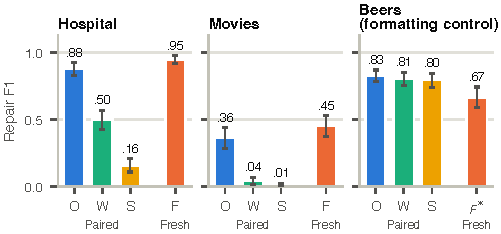
\includegraphics[width=\textwidth,height=.66\textheight,keepaspectratio]{../latex/figures/fig1_decomposition.pdf}
\caption{Four-condition DeepSeek-V4-Pro repair F1 on Hospital/Movies identity columns and all Beers columns, with original 95\% chunk-bootstrap intervals. F is unpaired; Beers F is descriptive.}
\label{report-fig-fig1_decomposition}
\end{figure}
\begin{figure}[!htbp]\centering
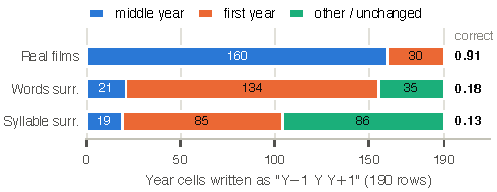
\includegraphics[width=\textwidth,height=.66\textheight,keepaspectratio]{../latex/figures/fig2_year_range.pdf}
\caption{Movies year candidates and repairs. Taking the middle candidate matches 167/190 references; the cleaner was not supplied this rule.}
\label{report-fig-fig2_year_range}
\end{figure}
\begin{figure}[!htbp]\centering
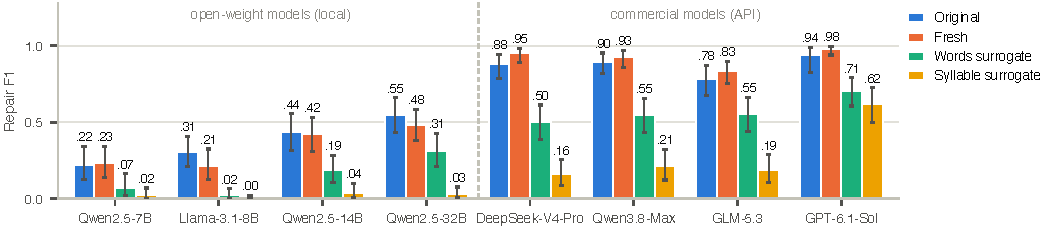
\includegraphics[width=\textwidth,height=.66\textheight,keepaspectratio]{../latex/figures/fig6_scale.pdf}
\caption{Full eight-model Hospital identity-column comparison with original 95\% chunk-bootstrap intervals. The scale trend is confined to the tested Qwen2.5 family on Hospital.}
\label{report-fig-fig6_scale}
\end{figure}
\begin{figure}[!htbp]\centering
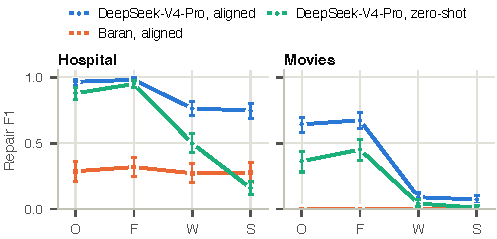
\includegraphics[width=\textwidth,height=.66\textheight,keepaspectratio]{../latex/figures/fig3_aligned.pdf}
\caption{Zero-shot and aligned repair F1. For aligned Baran only, whiskers are the first-run 95\% chunk-bootstrap interval translated to the three-run mean, not confidence intervals for that mean or seed ranges.}
\label{report-fig-fig3_aligned}
\end{figure}
\begin{figure}[!htbp]\centering
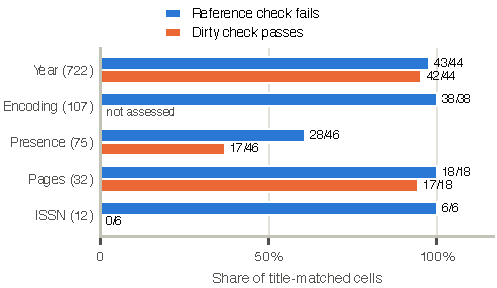
\includegraphics[width=\textwidth,height=.66\textheight,keepaspectratio]{../latex/figures/fig5_rayyan.pdf}
\caption{Original Rayyan stratified field-check display. The dirty changed-word check is unassessed. The plot uses the same saved matches and criteria as Section 3, not another sample.}
\label{report-fig-fig5_rayyan}
\end{figure}
\clearpage
\clearpage
\section{Archived sensitivity checks and output patterns}
\hypertarget{companion-7}{}\label{report-7}

We use the existing tables, replies and retrieval records to examine construction strength, incomplete replies, formatting repairs and title-match coverage. These diagnostics leave the main construction-seed-0 estimates, intervals and significance unchanged.

\subsection{Hospital construction strength}

Hospital's identity columns contain 219 erroneous cells. The original and all three word-surrogate tables have identical error positions. The acceptance check groups equal-length corruptions by the number of replaced characters and permits an eight-percentage-point difference in each bin.

\ensuretablespace{117pt}
\begingroup\setlength{\tabcolsep}{3pt}\renewcommand{\arraystretch}{1.18}
\footnotesize
\begin{longtable}{@{}>{\raggedright\arraybackslash}p{\dimexpr 0.2200\textwidth-5.10pt\relax}>{\raggedright\arraybackslash}p{\dimexpr 0.1560\textwidth-5.10pt\relax}>{\raggedright\arraybackslash}p{\dimexpr 0.1560\textwidth-5.10pt\relax}>{\raggedright\arraybackslash}p{\dimexpr 0.1560\textwidth-5.10pt\relax}>{\raggedright\arraybackslash}p{\dimexpr 0.1560\textwidth-5.10pt\relax}>{\raggedright\arraybackslash}p{\dimexpr 0.1560\textwidth-5.10pt\relax}@{}}
\caption{Hospital character-replacement strength distributions and acceptance outcomes.}\label{report-table-7-1}\\
\toprule
Table & One character & Two characters & Three or more & Maximum difference from O & Strength check \\
\midrule
\endfirsthead
\multicolumn{6}{l}{\small Table \thetable\ (continued)}\\
\toprule
Table & One character & Two characters & Three or more & Maximum difference from O & Strength check \\
\midrule
\endhead
\midrule\multicolumn{6}{r}{\footnotesize Continued on next page}\\\endfoot
\bottomrule\endlastfoot
O & 118 (53.9\%) & 64 (29.2\%) & 37 (16.9\%) & --- & Reference \\
W, seed 0 & 136 (62.1\%) & 69 (31.5\%) & 14 (6.4\%) & 10.5023 points & Outside tolerance \\
W, seed 1 & 123 (56.2\%) & 66 (30.1\%) & 30 (13.7\%) & 3.1963 points & Pass \\
W, seed 2 & 118 (53.9\%) & 74 (33.8\%) & 27 (12.3\%) & 4.5662 points & Pass \\
\end{longtable}\endgroup

Seed 0's largest difference is 10.5023 points, or 2.5023 points beyond the tolerance. Character counts describe the corruption distribution; they do not measure a cleaner's difficulty. The following comparison uses the two passing word-surrogate constructions, alongside the corresponding fresh and syllable constructions. Ranges span seeds 1 and 2, rather than bootstrap samples. Differences use the archived scorer's four-decimal condition scores, before rounding for display in the main tables.

\ensuretablespace{149pt}
\begingroup\setlength{\tabcolsep}{3pt}\renewcommand{\arraystretch}{1.18}
\small
\begin{longtable}{@{}>{\raggedright\arraybackslash}p{\dimexpr 0.2000\textwidth-4.90pt\relax}>{\raggedright\arraybackslash}p{\dimexpr 0.2000\textwidth-4.90pt\relax}>{\raggedright\arraybackslash}p{\dimexpr 0.2000\textwidth-4.90pt\relax}>{\raggedright\arraybackslash}p{\dimexpr 0.2000\textwidth-4.90pt\relax}>{\raggedright\arraybackslash}p{\dimexpr 0.2000\textwidth-4.90pt\relax}@{}}
\caption{Hospital condition-contrast ranges over passing word-surrogate seeds 1 and 2.}\label{report-table-7-2}\\
\toprule
Cleaner & O-W & F-W & W-S & O-S \\
\midrule
\endfirsthead
\multicolumn{5}{l}{\small Table \thetable\ (continued)}\\
\toprule
Cleaner & O-W & F-W & W-S & O-S \\
\midrule
\endhead
\midrule\multicolumn{5}{r}{\footnotesize Continued on next page}\\\endfoot
\bottomrule\endlastfoot
DeepSeek-V4-Pro & .3166--.3303 & .3395--.3690 & .3331--.3604 & .6634--.6770 \\
Qwen3.8-Max & .3102--.3192 & .3372--.3444 & .3628--.3814 & .6820--.6916 \\
GLM-5.3 & .2153--.2623 & .2764--.2865 & .3436--.3555 & .5708--.6059 \\
GPT-6.1-Sol & .2333--.2406 & .2764--.2919 & .0993--.1048 & .3381--.3399 \\
Qwen2.5-7B & .1335--.1712 & .1876--.2197 & .0222--.0664 & .1934--.1999 \\
Llama-3.1-8B & .2511--.2921 & .1364--.2360 & .0098--.0440 & .2951--.3019 \\
Qwen2.5-14B & .2517--.2576 & .3057--.3141 & .1169--.1669 & .3745--.4186 \\
Qwen2.5-32B & .2115--.2466 & .2366--.2996 & .2698--.2804 & .4919--.5164 \\
\end{longtable}\endgroup

All eight cleaners retain positive F-W and W-S contrasts in these constructions. O-S does not involve W. Together with the all-seed ranges in the paper, these results separate the seed-0 strength exception from the persistence of the observed direction across existing constructions.

\subsection{Incomplete Movies replies}

GLM-5.3 has eight incomplete replies among 500 chunks over ten Movies tables: O and three seeds each of F, W and S. Six occur in the four seed-0 tables. The table includes zero counts to make that scope explicit; chunk numbers are one-based within a table.

\ensuretablespace{170pt}
\begingroup\setlength{\tabcolsep}{3pt}\renewcommand{\arraystretch}{1.18}
\small
\begin{longtable}{@{}>{\raggedright\arraybackslash}p{\dimexpr 0.2200\textwidth-4.10pt\relax}>{\raggedright\arraybackslash}p{\dimexpr 0.1400\textwidth-4.10pt\relax}>{\raggedright\arraybackslash}p{\dimexpr 0.6400\textwidth-4.10pt\relax}@{}}
\caption{GLM-5.3 incomplete Movies replies across the ten archived tables.}\label{report-table-7-3}\\
\toprule
Condition & Incomplete / 50 & Chunk numbers \\
\midrule
\endfirsthead
\multicolumn{3}{l}{\small Table \thetable\ (continued)}\\
\toprule
Condition & Incomplete / 50 & Chunk numbers \\
\midrule
\endhead
\midrule\multicolumn{3}{r}{\footnotesize Continued on next page}\\\endfoot
\bottomrule\endlastfoot
O & 1 & 24 \\
F, seed 0 & 0 & --- \\
F, seed 1 & 0 & --- \\
F, seed 2 & 0 & --- \\
W, seed 0 & 1 & 47 \\
W, seed 1 & 0 & --- \\
W, seed 2 & 0 & --- \\
S, seed 0 & 4 & 14, 16, 26, 47 \\
S, seed 1 & 0 & --- \\
S, seed 2 & 2 & 14, 47 \\
\end{longtable}\endgroup

Every incomplete reply contains only {\ttfamily\small \{"}, yielding no parsed corrections. Incompleteness is identified by the archived client's delimiter heuristic, not an archived provider termination reason. The main scores count these replies as no corrections.

For the exclusion check, O-W removes a paired chunk if either reply is incomplete, retaining 48 common pairs. F-W removes incomplete replies independently, retaining 50 fresh chunks and 49 word-surrogate chunks. Both versions use 2,000 bootstrap resamples and seed 0, with the original pairing rules and the original 40-comparison Holm family (eight cleaners \(\times\) five Hospital/Movies contrasts).

\ensuretablespace{106pt}
\begingroup\setlength{\tabcolsep}{3pt}\renewcommand{\arraystretch}{1.18}
\small
\begin{longtable}{@{}>{\raggedright\arraybackslash}p{\dimexpr 0.2000\textwidth-4.90pt\relax}>{\raggedright\arraybackslash}p{\dimexpr 0.2000\textwidth-4.90pt\relax}>{\raggedright\arraybackslash}p{\dimexpr 0.2000\textwidth-4.90pt\relax}>{\raggedright\arraybackslash}p{\dimexpr 0.2000\textwidth-4.90pt\relax}>{\raggedright\arraybackslash}p{\dimexpr 0.2000\textwidth-4.90pt\relax}@{}}
\caption{GLM-5.3 Movies contrasts before and after incomplete-reply exclusion.}\label{report-table-7-4}\\
\toprule
GLM Movies comparison & Replies included & Chunks, left/right & Difference & 95\% percentile interval \\
\midrule
\endfirsthead
\multicolumn{5}{l}{\small Table \thetable\ (continued)}\\
\toprule
GLM Movies comparison & Replies included & Chunks, left/right & Difference & 95\% percentile interval \\
\midrule
\endhead
\midrule\multicolumn{5}{r}{\footnotesize Continued on next page}\\\endfoot
\bottomrule\endlastfoot
F-W & All & 50 / 50 & .1660 & [.1046, .2268] \\
F-W & Complete only & 50 / 49 & .1654 & [.1044, .2292] \\
O-W & All & 50 / 50 & .0698 & [.0283, .1112] \\
O-W & Complete pairs & 48 / 48 & .0680 & [.0263, .1119] \\
\end{longtable}\endgroup

Both contrasts remain significant under the original Holm procedure in the sensitivity family. The other 38 comparisons, including their adjusted values, are unchanged. For these two contrasts, the archived Monte Carlo tail calculation returns zero in both versions: no sampled tail events, rather than a population probability of zero. Intervals are unadjusted percentile intervals. The diagnostic aggregate described in Section 7.7 records all 40 comparisons in their original order for each version.

\subsection{Rating-count repairs}

DeepSeek-V4-Pro's Movies replies show a different pattern on rating counts than on years. The dirty and reference rating-count columns are identical across O/W/S. Repairs of these counts are all exact comma deletions, but the model applies the transformation unevenly.

\ensuretablespace{240pt}
\begingroup\setlength{\tabcolsep}{3pt}\renewcommand{\arraystretch}{1.18}
\footnotesize
\begin{longtable}{@{}>{\raggedright\arraybackslash}p{\dimexpr 0.0900\textwidth-5.43pt\relax}>{\raggedright\arraybackslash}p{\dimexpr 0.1138\textwidth-5.43pt\relax}>{\raggedright\arraybackslash}p{\dimexpr 0.1138\textwidth-5.43pt\relax}>{\raggedright\arraybackslash}p{\dimexpr 0.1138\textwidth-5.43pt\relax}>{\raggedright\arraybackslash}p{\dimexpr 0.1138\textwidth-5.43pt\relax}>{\raggedright\arraybackslash}p{\dimexpr 0.1138\textwidth-5.43pt\relax}>{\raggedright\arraybackslash}p{\dimexpr 0.1138\textwidth-5.43pt\relax}>{\raggedright\arraybackslash}p{\dimexpr 0.1138\textwidth-5.43pt\relax}>{\raggedright\arraybackslash}p{\dimexpr 0.1138\textwidth-5.43pt\relax}@{}}
\caption{DeepSeek-V4-Pro Movies rating-count proposals, effective edits, and repairs.}\label{report-table-7-5}\\
\toprule
Condition & Error cells & Raw proposals & No-op proposals & Effective edits & Repairs & Wrong edits on error cells & Correct cells modified & Error cells without effective edits \\
\midrule
\endfirsthead
\multicolumn{9}{l}{\small Table \thetable\ (continued)}\\
\toprule
Condition & Error cells & Raw proposals & No-op proposals & Effective edits & Repairs & Wrong edits on error cells & Correct cells modified & Error cells without effective edits \\
\midrule
\endhead
\midrule\multicolumn{9}{r}{\footnotesize Continued on next page}\\\endfoot
\bottomrule\endlastfoot
O & 768 & 80 & 73 & 7 & 2 & 1 & 4 & 765 \\
F & 1,000 & 69 & 43 & 26 & 26 & 0 & 0 & 974 \\
W & 768 & 170 & 117 & 53 & 24 & 8 & 21 & 736 \\
S & 768 & 313 & 190 & 123 & 90 & 16 & 17 & 662 \\
\end{longtable}\endgroup

All listed proposals have valid row and column addresses. No-op proposals equal the dirty value under the scorer's case/whitespace normalization and do not count as edits. Repeated proposals retain the last effective edit; a later no-op does not erase it. The 200 chunk-level results agree with the original scoring function.

The 90 S repairs occur in seven chunks: 2 (18 repairs), 15 (18), 21 (8), 31 (15), 41 (15), 48 (1), and 50 (15). O repairs occur in two chunks, W repairs in five and F repairs in three. Thus the S increase is concentrated in a subset of replies, rather than a uniform improvement over all chunks. The output evidence shows variable use of an available formatting rule; it does not identify the model's internal reason for selecting that rule.

\subsection{Rayyan title-matching coverage}

The 279 sampled cells yield 152 title-matched cells (152/279 = 54.5\%), associated with 121 distinct PMIDs. Field-specific match rates and checks are as follows. A dash means that the dirty field was not assessed, rather than a failed check.

\ensuretablespace{127pt}
\begingroup\setlength{\tabcolsep}{3pt}\renewcommand{\arraystretch}{1.18}
\footnotesize
\begin{longtable}{@{}>{\raggedright\arraybackslash}p{\dimexpr 0.2200\textwidth-5.10pt\relax}>{\raggedright\arraybackslash}p{\dimexpr 0.1560\textwidth-5.10pt\relax}>{\raggedright\arraybackslash}p{\dimexpr 0.1560\textwidth-5.10pt\relax}>{\raggedright\arraybackslash}p{\dimexpr 0.1560\textwidth-5.10pt\relax}>{\raggedright\arraybackslash}p{\dimexpr 0.1560\textwidth-5.10pt\relax}>{\raggedright\arraybackslash}p{\dimexpr 0.1560\textwidth-5.10pt\relax}@{}}
\caption{Rayyan cell-level title-matching coverage and matched field outcomes.}\label{report-table-7-6}\\
\toprule
Field type & Sampled & Matched & Match rate & Matched dirty fields passing & Matched reference fields passing \\
\midrule
\endfirsthead
\multicolumn{6}{l}{\small Table \thetable\ (continued)}\\
\toprule
Field type & Sampled & Matched & Match rate & Matched dirty fields passing & Matched reference fields passing \\
\midrule
\endhead
\midrule\multicolumn{6}{r}{\footnotesize Continued on next page}\\\endfoot
\bottomrule\endlastfoot
Date & 80 & 44 & 55.0\% & 42 / 44 & 1 / 44 \\
Encoding & 80 & 38 & 47.5\% & --- & 0 / 38 \\
Missing volume/issue & 75 & 46 & 61.3\% & 17 / 46 & 18 / 46 \\
Pagination & 32 & 18 & 56.3\% & 17 / 18 & 0 / 18 \\
ISSN & 12 & 6 & 50.0\% & 0 / 6 & 0 / 6 \\
\end{longtable}\endgroup

Dates are checked against publication year, volume/issue against presence, pagination against the page string, ISSN against print or electronic identifiers, and encoding against the changed-word criterion in the paper. The weighted reference-check failure rate remains 95.2\% [91.2\%, 97.8\%], using matched cells within each type and the 948-cell type composition for weights. Its interval conditions on the saved matches and checks. Unmatched cells receive no new field judgments. Matching and field semantics are detailed in \hyperlink{companion-3}{Rayyan audit criteria (Section~\ref{report-3})}.

\subsection{Exact direct-editing prompt}

The following literals come from the archived cleaning source. They specify the zero-shot direct-editing task, not the continuation or conflict prompts. Python's doubled braces escape literal JSON braces; {\ttfamily\small \{block\}} is replaced by the input CSV, including its {\ttfamily\small \_\allowbreak{}row} column.

System message:

\begin{quote}
\begin{Verbatim}[fontsize=\footnotesize,fontfamily=cmtt,formatcom={\fontencoding{OT1}\selectfont\def\textasciigrave{\char18}\def\textquotesingle{\char13}}]
You are a meticulous data cleaning assistant. Reply with JSON only.
\end{Verbatim}
\end{quote}

User-message template:

\begin{quote}
\begin{Verbatim}[fontsize=\footnotesize,fontfamily=cmtt,formatcom={\fontencoding{OT1}\selectfont\def\textasciigrave{\char18}\def\textquotesingle{\char13}}]
The CSV table below contains some erroneous cells (for example typos or corrupted values). The first
column `_row` numbers the rows.
Find the erroneous cells and give their correct values. Only list cells you believe are wrong; do
not rewrite correct cells.
Reply with JSON: {{"corrections": [{{"row": <_row>, "column": "<column name>", "value": "<corrected
value>"}}]}}

{block}
\end{Verbatim}
\end{quote}

\subsection{Recorded token usage}

The historical usage log contains 11,413 entries, including entries not assigned to the paper's final workloads. Its input and output totals are reported separately below. Reasoning tokens are already included in output tokens and must not be added again.

\ensuretablespace{138pt}
\begingroup\setlength{\tabcolsep}{3pt}\renewcommand{\arraystretch}{1.18}
\footnotesize
\begin{longtable}{@{}>{\raggedright\arraybackslash}p{\dimexpr 0.2200\textwidth-5.10pt\relax}>{\raggedright\arraybackslash}p{\dimexpr 0.1560\textwidth-5.10pt\relax}>{\raggedright\arraybackslash}p{\dimexpr 0.1560\textwidth-5.10pt\relax}>{\raggedright\arraybackslash}p{\dimexpr 0.1560\textwidth-5.10pt\relax}>{\raggedright\arraybackslash}p{\dimexpr 0.1560\textwidth-5.10pt\relax}>{\raggedright\arraybackslash}p{\dimexpr 0.1560\textwidth-5.10pt\relax}@{}}
\caption{Historical usage-log totals; reasoning tokens are included in output tokens.}\label{report-table-7-7}\\
\toprule
Logged model & Entries & Input tokens & Output tokens & Known reasoning tokens within output & Entries with unknown reasoning count \\
\midrule
\endfirsthead
\multicolumn{6}{l}{\small Table \thetable\ (continued)}\\
\toprule
Logged model & Entries & Input tokens & Output tokens & Known reasoning tokens within output & Entries with unknown reasoning count \\
\midrule
\endhead
\midrule\multicolumn{6}{r}{\footnotesize Continued on next page}\\\endfoot
\bottomrule\endlastfoot
DeepSeek-V4-Pro & 3,169 & 7,512,112 & 2,615,556 & 0 & 0 \\
Qwen3.8-Max & 2,953 & 4,931,264 & 654,694 & 0 & 0 \\
GLM-5.3 & 2,806 & 3,971,489 & 2,984,507 & 2,565,488 & 0 \\
Gemini-3.5-Flash & 12 & 23,830 & 3,240 & Unknown & 12 \\
GPT-6.1-Sol & 2,473 & 3,320,127 & 588,719 & 295,011 & 0 \\
Total & 11,413 & 19,758,822 & 6,846,716 & 2,860,499 known & 12 \\
\end{longtable}\endgroup

These are usage-log totals, not the total tokens or monetary cost of the study. The log can contain retries and pilots; attribution to final experiments and coverage of local or cached runs are not established. Gemini entries describe historical usage and do not add a model to the eight-cleaner evaluation. The archived material does not establish the actual monetary fees. Request settings and the approximately 23,000-prompt workload breakdown remain in \hyperlink{companion-2}{Run and scoring specification (Section~\ref{report-2})}.

\subsection{Traceability and offline verification}

The diagnostic aggregate contains the diagnostics, exact prompt literals and SHA-256 bindings for 184 source files. Its SHA-256 is {\ttfamily\small f29316b0\allowbreak{}f90fd0e4\allowbreak{}3345f1ad\allowbreak{}80a4fbb3\allowbreak{}c9e48c95\allowbreak{}2748e95d\allowbreak{}42fcde33\allowbreak{}77192e34}. This historical source index records author-side provenance, not a claim that all 184 sources are redistributed. The repository's \href{https://github.com/hinsonver/CoRe-Benchmark/blob/main/tools/review_diagnostics.py}{\nolinkurl{tools/review_diagnostics.py}} and \href{https://github.com/hinsonver/CoRe-Benchmark/blob/main/docs/reproduction.md}{\nolinkurl{docs/reproduction.md}} distinguish replayable checks from aggregate-only output-pattern and usage evidence.

From the repository root:

\begin{quote}
\begin{Verbatim}[fontsize=\footnotesize,fontfamily=cmtt,formatcom={\fontencoding{OT1}\selectfont\def\textasciigrave{\char18}\def\textquotesingle{\char13}}]
python3 tools/review_diagnostics.py
\end{Verbatim}
\end{quote}

The original author-side audit read archived inputs, extracted pure scoring definitions and literal templates, and checked masks, replies, pairing, the full Holm family and parity with the original scorer. The repository replay recomputes the checks supported by included tables, block-count witnesses and saved matches. It reports aggregate-only evidence separately, without reconstructing omitted Movies replies or the historical billing log. Neither route invokes model generation.
\end{document}
